

\tikzset{every picture/.style={line width=0.75pt}} %set default line width to 0.75pt        

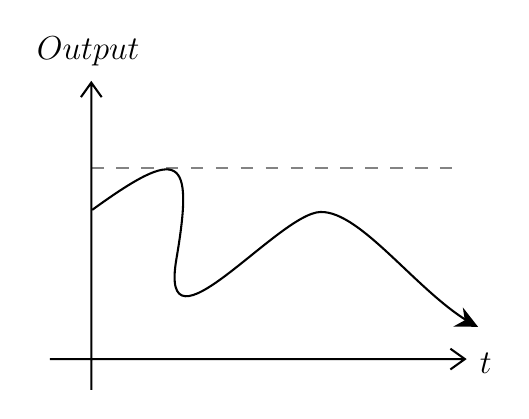
\begin{tikzpicture}[x=0.75pt,y=0.75pt,yscale=-1,xscale=1]
%uncomment if require: \path (0,300); %set diagram left start at 0, and has height of 300

%Straight Lines [id:da45173516768188793] 
\draw [color={rgb, 255:red, 131; green, 131; blue, 131 }  ,draw opacity=1 ] [dash pattern={on 4.5pt off 4.5pt}]  (110,131.33) -- (290,131.33) ;


%Shape: Axis 2D [id:dp17702348361548204] 
\draw  (90,223.2) -- (290,223.2)(110,90) -- (110,238) (283,218.2) -- (290,223.2) -- (283,228.2) (105,97) -- (110,90) -- (115,97)  ;
%Curve Lines [id:da6473783232781454] 
\draw    (110.42,151.33) .. controls (152.75,120.66) and (159.67,124.33) .. (151,174.99) .. controls (142.33,225.66) and (200,152.99) .. (220.33,152.33) .. controls (240.26,151.67) and (268.19,192.64) .. (294.71,206.83) ;
\draw [shift={(296.33,207.66)}, rotate = 206.28] [fill={rgb, 255:red, 0; green, 0; blue, 0 }  ][line width=0.75]  [draw opacity=0] (10.72,-5.15) -- (0,0) -- (10.72,5.15) -- (7.12,0) -- cycle    ;


% Text Node
\draw (108.5,75) node   {\large $Output$};
% Text Node
\draw (300,225) node   {\large $t$};


\end{tikzpicture}
